\newpage
\section*{Figures}

\begin{figure}[ht!]\centering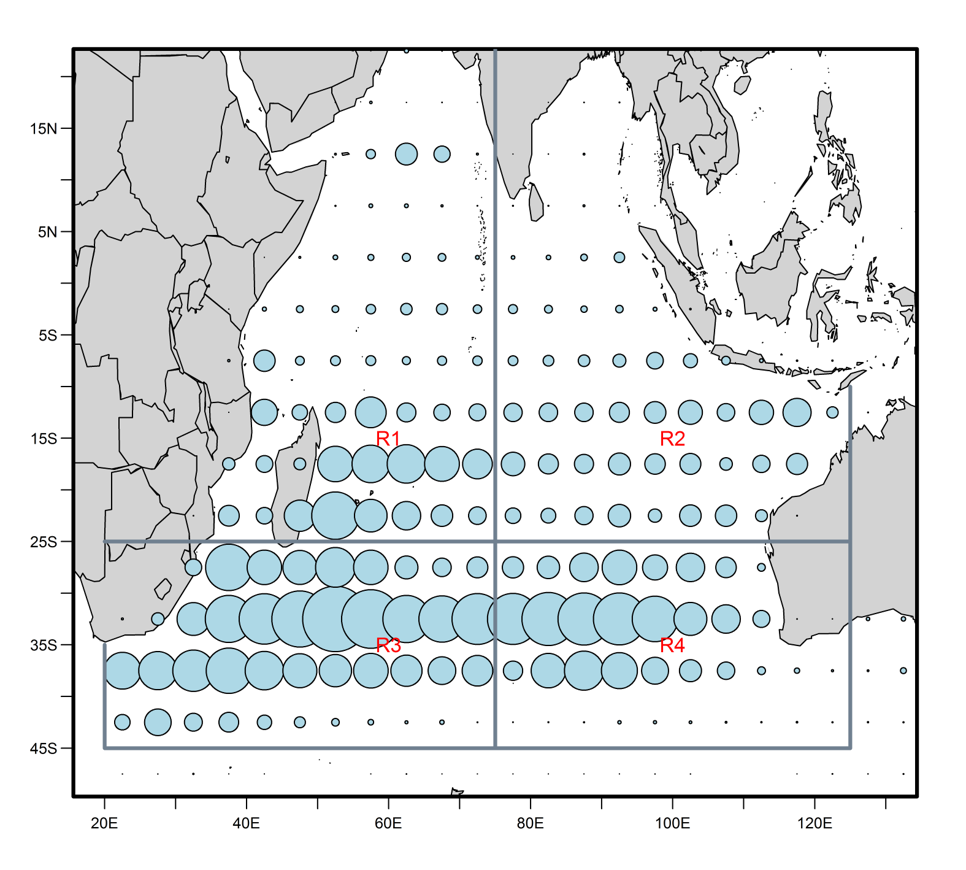
\includegraphics[width=0.75\textwidth]{figures/alb-map.png} 
\caption{Distribution of Indian Ocean albacore tuna catches by assessment areas.}
\label{fig:map}
\end{figure}

\begin{figure}[ht!]\centering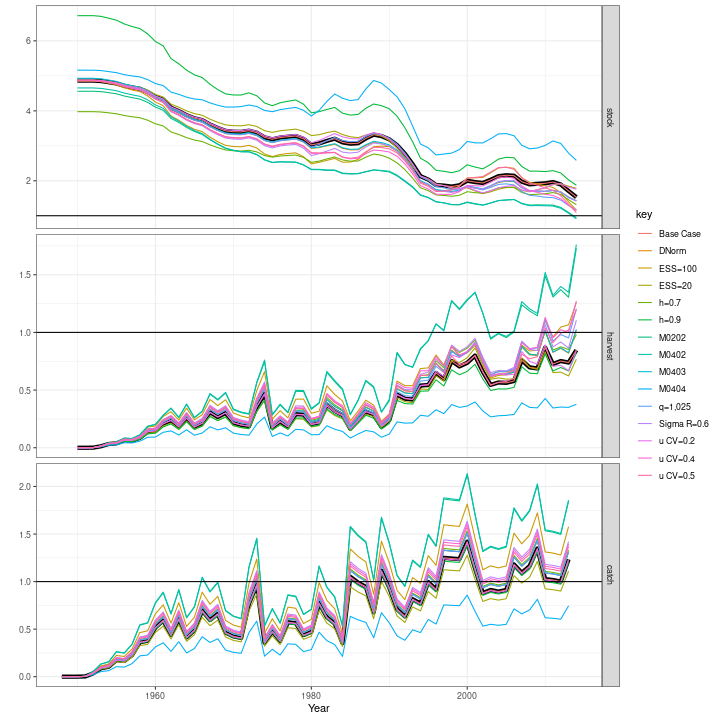
\includegraphics[width=0.75\textwidth]{figures/main-trends-1.png} \caption{Time series of spawning stock biomass and fishing mortality relative to $MSY$ target reference points for the main effects of the Indian Ocean albacore tuna assessment model grid.}
\label{fig:ts}
\end{figure}

\begin{figure}[ht!]\centering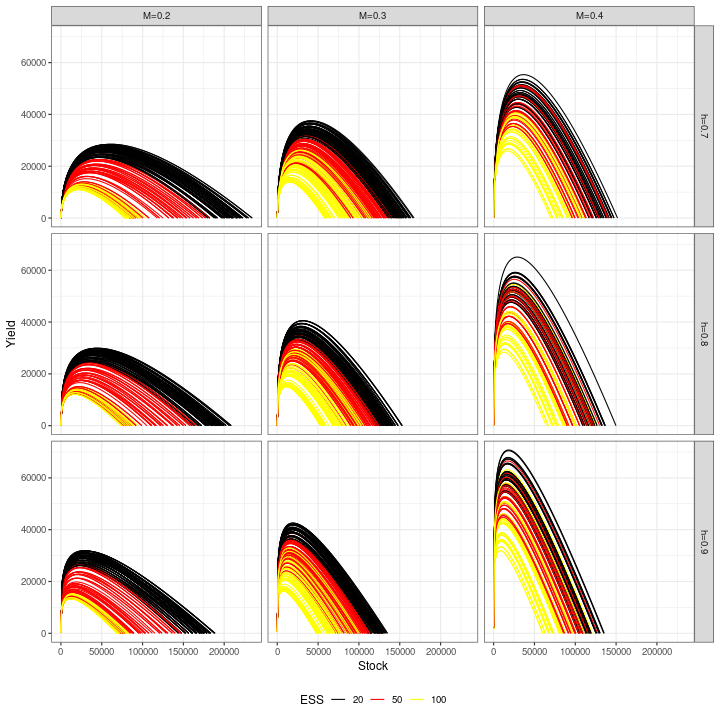
\includegraphics[width=0.75\textwidth]{figures/pf-grid-1.png} 
\caption{Production by steepness and mature natural mortality}
\label{fig:pf}       
\end{figure}

\begin{figure}
        \begin{subfigure}[b]{0.5\textwidth}
               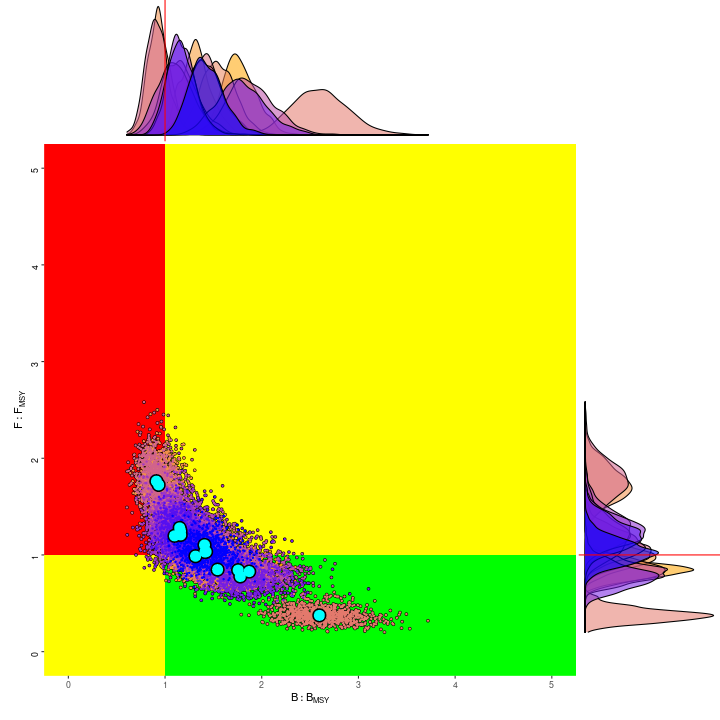
\includegraphics[width=\linewidth]{figures/kobe-main-1.png}
                \caption{Main effects with estimation error.}
                \label{fig:kobe-main}
        \end{subfigure}%
                \begin{subfigure}[b]{0.5\textwidth}
                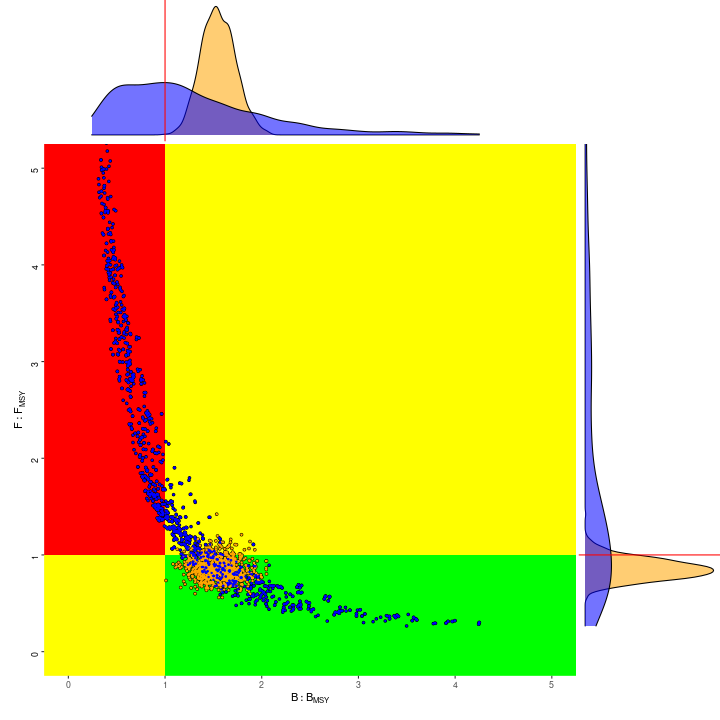
\includegraphics[width=\linewidth]{figures/kobe-bg-1.png}
                \caption{Reference case and grid with model.}
                \label{fig:kobe-bg}
        \end{subfigure}%
        \caption{Kobe phase plots showing spawning biomass ($B$) and fishing mortality ($F$) relative to $MSY$ target reference points. Within model uncertainty was approximating using multivariate log-normal distribution derived from Hessian matrix (MVLN) with cyan points denoting the median}\label{fig:kobe}
\end{figure}

\clearpage
\newpage
\begin{figure}[ht!]\centering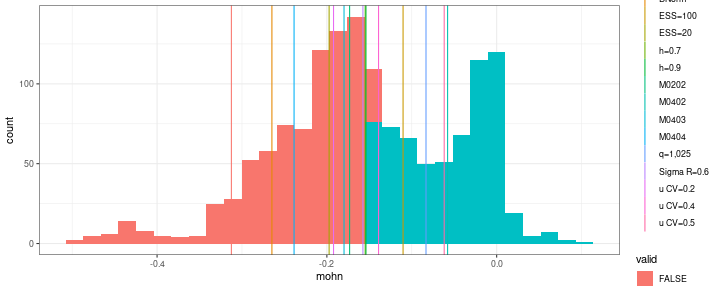
\includegraphics[width=0.75\textwidth]{figures/mohn3-1.png}  \caption{Summary of Mohn's $\rho$ for the for the 1440 assessment models in the Indian Ocean albacore tuna grid, with main effects indicated by the vertical lines.} 
\label{fig:mohn}       
\end{figure}

\begin{figure}
    \begin{subfigure}[a]{0.35\textwidth}
    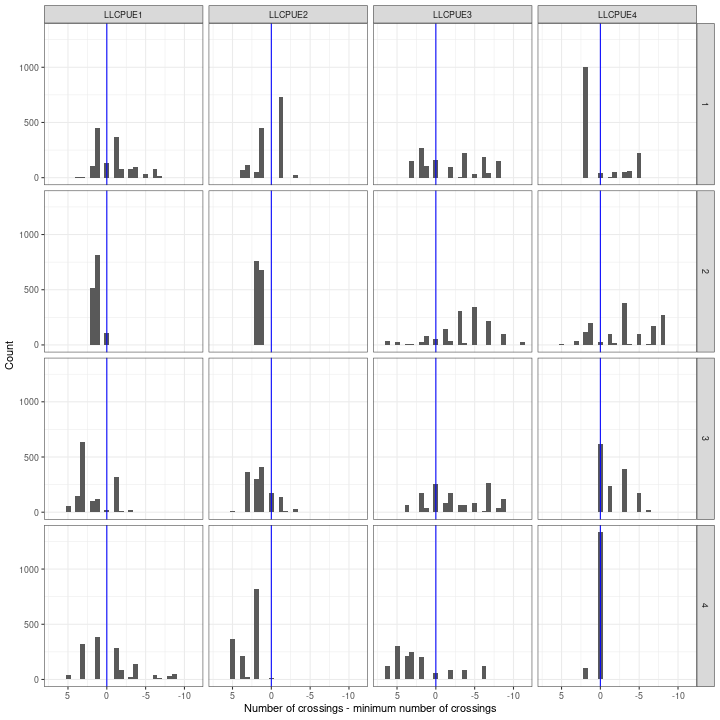
\includegraphics[width=\linewidth]{figures/run-cross-1.png}
    \caption{Number of crossings - minimum expected number of crossings; note reversed x-axis.}
    \label{fig:runs-cross} 
    \end{subfigure}%
    \begin{subfigure}[b]{0.35\textwidth}
    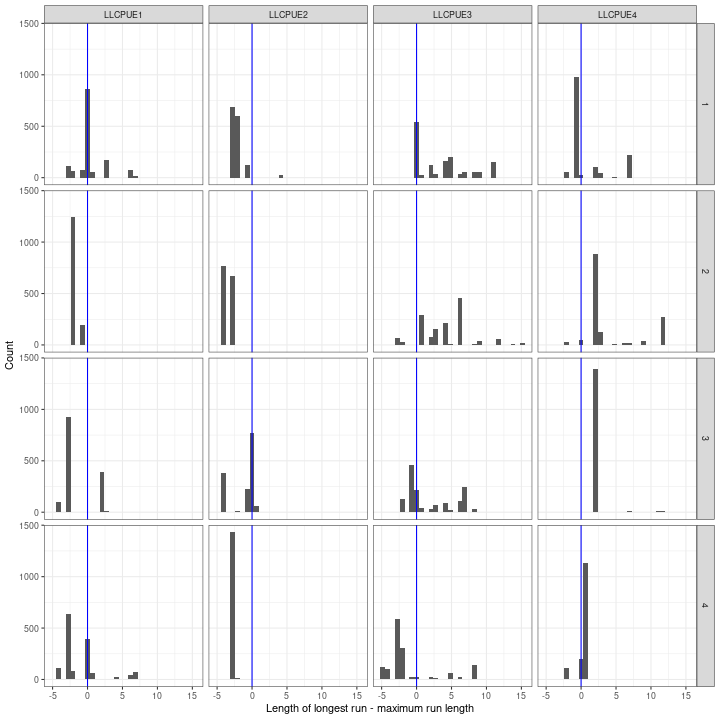
\includegraphics[width=\linewidth]{figures/run-long-1.png}
    \caption{Longest run - maximum expected run length.}
    \label{fig:runs-long}
    \end{subfigure}%
    \begin{subfigure}[c]{0.35\textwidth}
    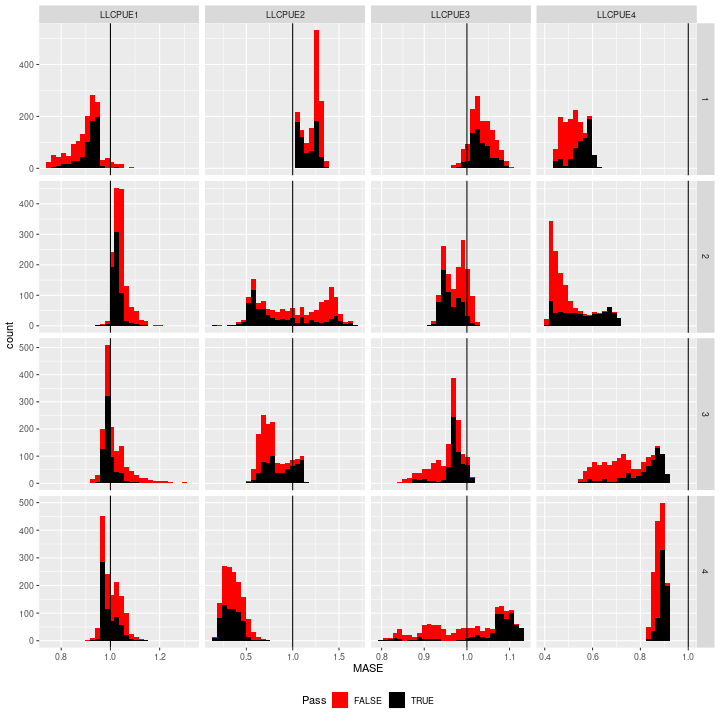
\includegraphics[width=\linewidth]{figures/mase-1.png}
    \caption{MASE.}
    \label{fig:mase}
    \end{subfigure}%
 
\caption{}\label{fig:runs}
\end{figure}


%\begin{figure}[ht!]\centering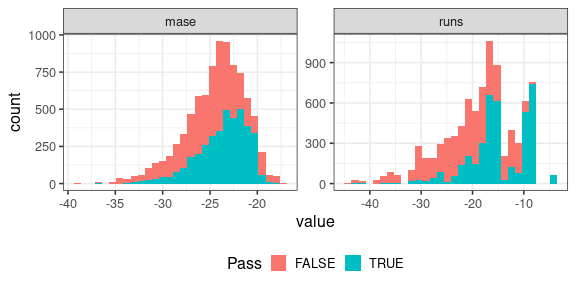
\includegraphics[width=0.75\textwidth]{figures/cf-1.png} \caption{Summary of weighting diagnostics.}\label{fig:wts} \end{figure}

\begin{figure}[ht!]\centering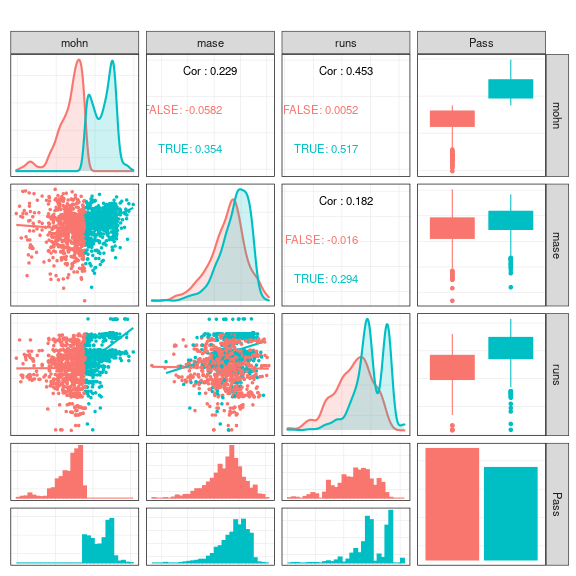
\includegraphics[width=0.75\textwidth]{figures/ggpair-1.png} \caption{Correlations between weighting diagnostics.}
\label{fig:wts}       
\end{figure}

\newpage
\begin{figure}[!ht]
	\centering
	\begin{subfigure}{0.9\textwidth}
		\centering
		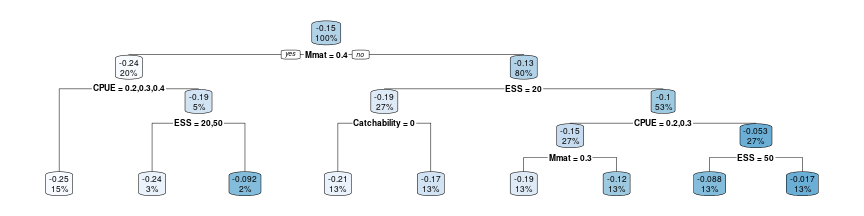
\includegraphics[width=\textwidth]{figures/a-tree-1.png}
		\caption{Regression Tree}
		\label{fig:tree}
	\end{subfigure}
	\hfill
	\begin{subfigure}{0.9\textwidth}  
		\centering 
		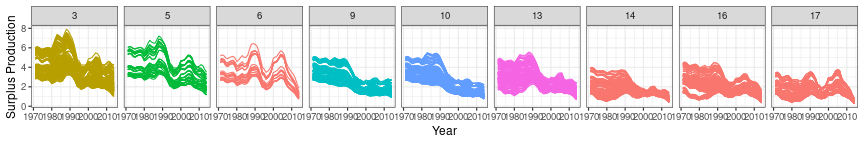
\includegraphics[width=\textwidth]{figures/a-tree-biomass-1.png}
		\caption{SSB}
		\label{fig:tree-b}
	\end{subfigure}
	\begin{subfigure}{0.9\textwidth}  
		\centering 
		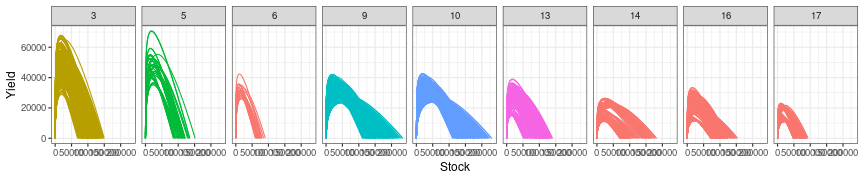
\includegraphics[width=\textwidth]{figures/a-tree-pf-1.png}
		\caption{Production Function}
		\label{fig:tree-pf}
	\end{subfigure}
	\begin{subfigure}{0.9\textwidth}
		\centering
	    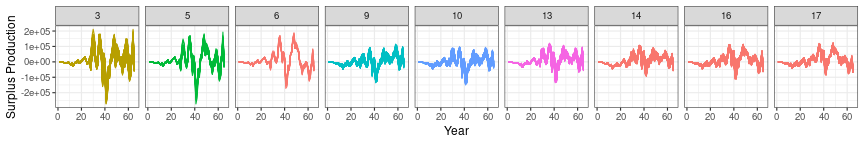
\includegraphics[width=\textwidth]{figures/a-tree-sp-1.png}
		\caption{Surplus Production}
		\label{fig:tree-sp}
	\end{subfigure}
	\caption{Mohn's $\rho$}
	\label{fig:tree}
\end{figure}


\begin{figure}
        \begin{subfigure}[b]{0.5\textwidth}
                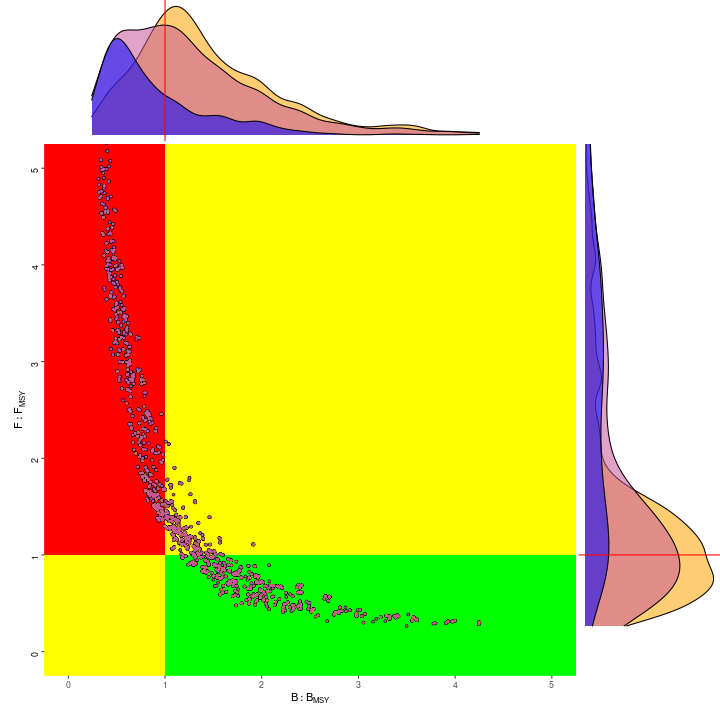
\includegraphics[width=\linewidth]{figures/kobe-mohn3-2.png}
                \caption{Kobe}
                \label{fig:kobe-wt}
        \end{subfigure}%
        \begin{subfigure}[b]{0.5\textwidth}
                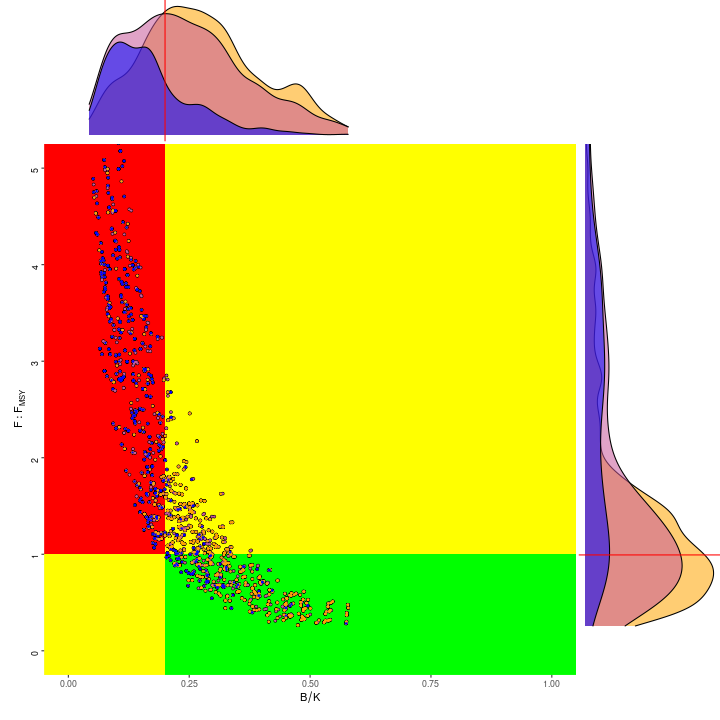
\includegraphics[width=\linewidth]{figures/majuro-mohn3-all-1.png}
                \caption{Majuro}
                \label{fig:majuro-wt}
        \end{subfigure}%
        \caption{Phase plots for all 1440 grid models, with equal, AIC, and skill weighting identifying models that pass the Mohn's $\rho$ test for hindcasts with 3 year ahead forecasts .}
        \label{fig:phase-wt}
\end{figure}


%\begin{figure}[ht!]\centering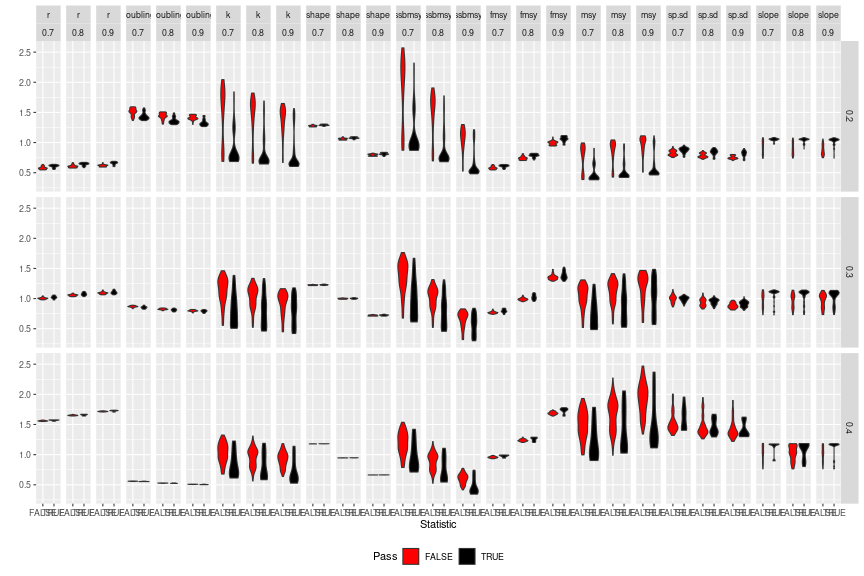
\includegraphics[width=1\textwidth]{figures/param-box-mohn3-1.png}\caption{Summary statistics, will re-do for $F/F_{MSY}$, $B/B_{MSY}$, $r$, $K$, $p$ and $sd(sp)$, and population doubling time.}\label{fig:smry}\end{figure}

\newpage
\begin{figure}[!ht]
	\centering
	\begin{subfigure}{0.32\textwidth}
		\centering
		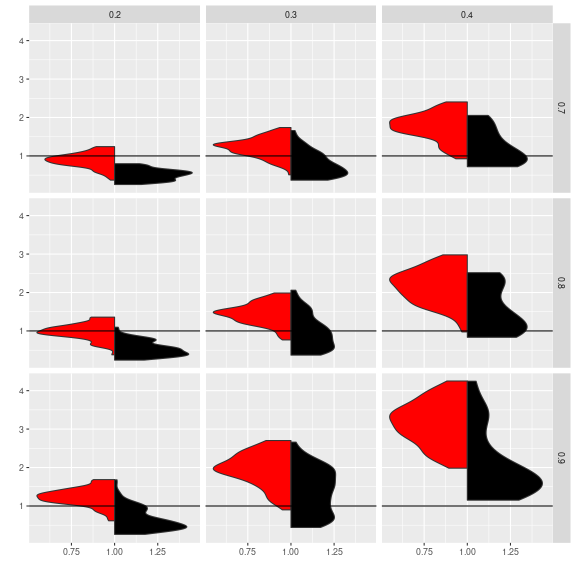
\includegraphics[width=\textwidth]{figures/v-b-1.png}
		\caption{$SSB/B_{MSY}$}
		\label{fig:grid-bmsy}
	\end{subfigure}
	\begin{subfigure}{0.32\textwidth}  
		\centering 
		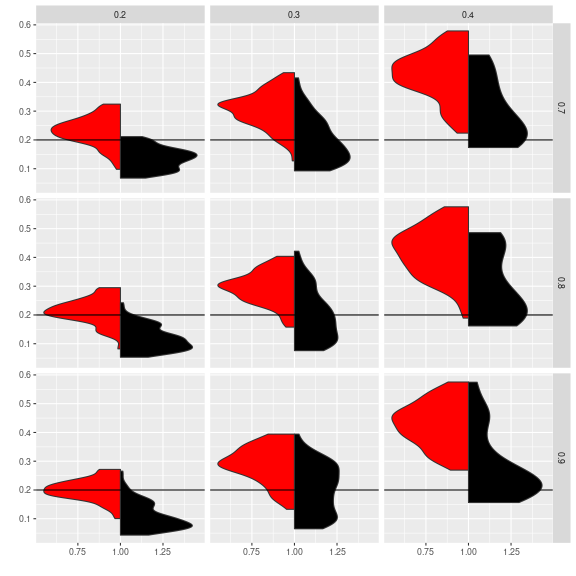
\includegraphics[width=\textwidth]{figures/v-m-1.png}
		\caption{$SSB/K$}
		\label{fig:grid-blim}
	\end{subfigure}
	\begin{subfigure}{0.32\textwidth}  
		\centering 
		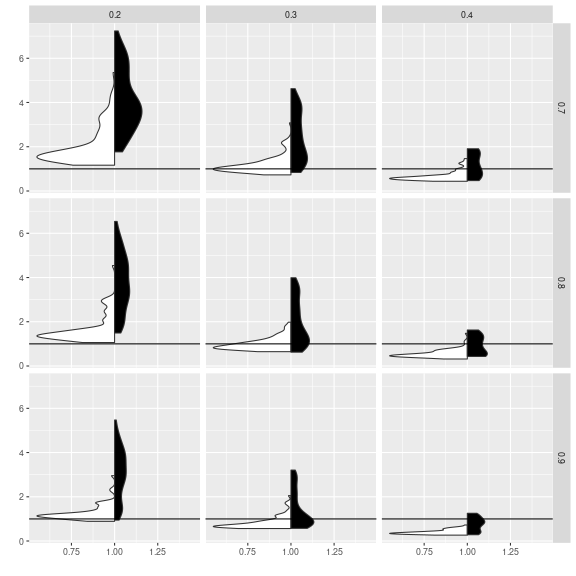
\includegraphics[width=\textwidth]{figures/v-h-1.png}
		\caption{$F/F_{MSY}$}
		\label{fig:grid-fmsy}
	\end{subfigure}
	\begin{subfigure}{0.32\textwidth}  
		\centering 
		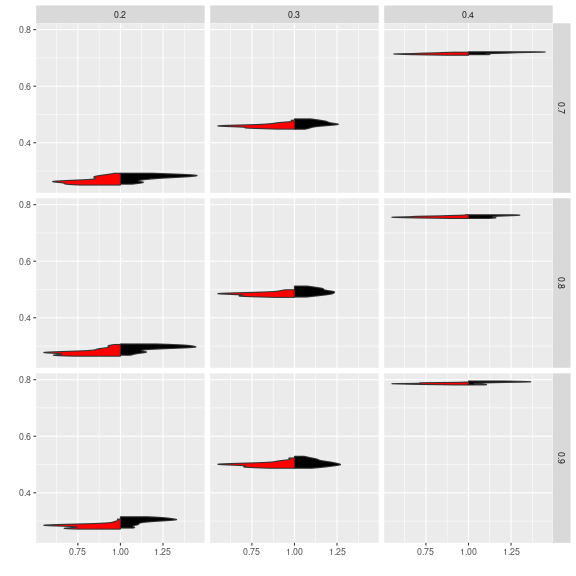
\includegraphics[width=\textwidth]{figures/v-r-1.png}
		\caption{$r$}
		\label{fig:grid-r}
	\end{subfigure}	\begin{subfigure}{0.32\textwidth}  
		\centering 
		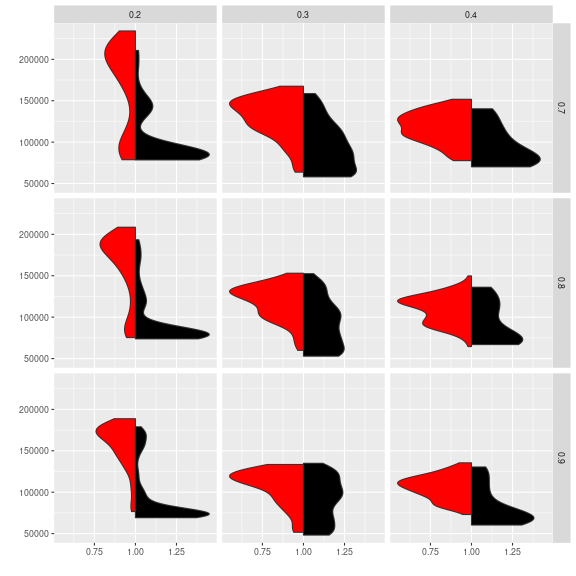
\includegraphics[width=\textwidth]{figures/v-k-1.png}
		\caption{$K$}
		\label{fig:grid-k}
	\end{subfigure}	\begin{subfigure}{0.32\textwidth}  
		\centering 
		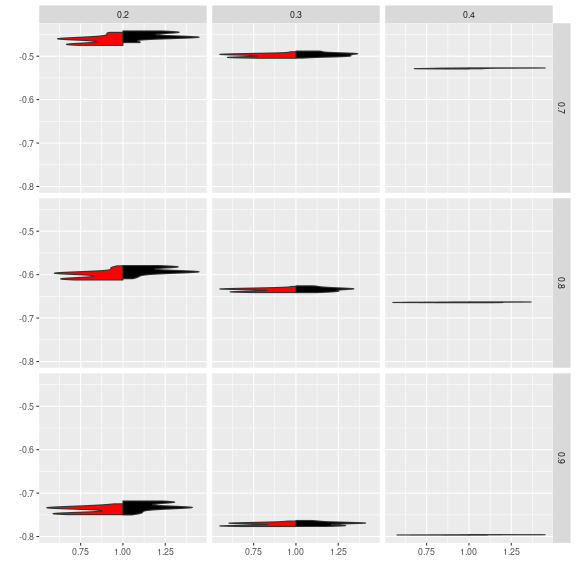
\includegraphics[width=\textwidth]{figures/v-p-1.png}
		\caption{$p$}
		\label{fig:grid-p}
	\end{subfigure}
	\begin{subfigure}{0.32\textwidth}  
		\centering 
		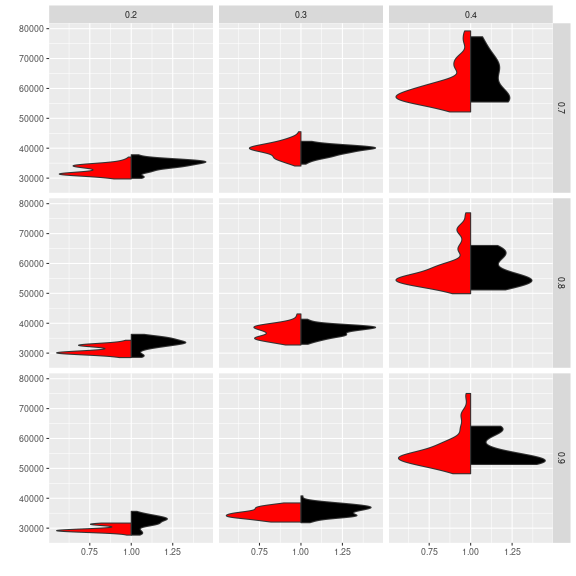
\includegraphics[width=\textwidth]{figures/v-sp-1.png}
		\caption{$sd(sp)$}
		\label{fig:grid-sp}
	\end{subfigure}	\begin{subfigure}{0.32\textwidth}  
		\centering 
		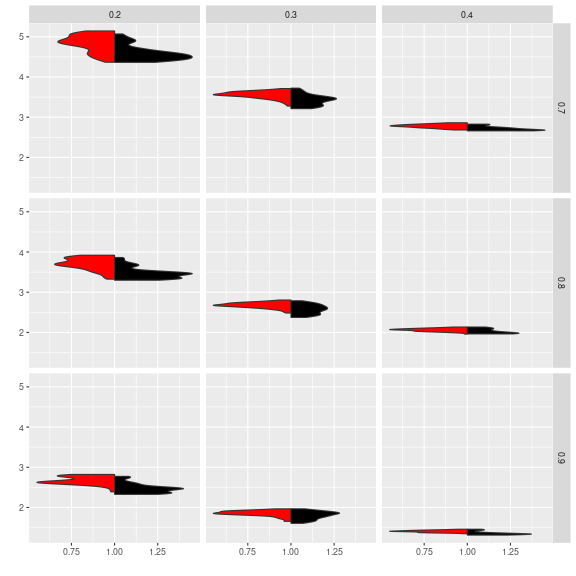
\includegraphics[width=\textwidth]{figures/v-d-1.png}
		\caption{Population doubling time}
		\label{fig:grid-dt}
	\end{subfigure}
	\caption{}
	\label{ref:grid}
\end{figure}

\iffalse
\begin{figure}[ht!]\centering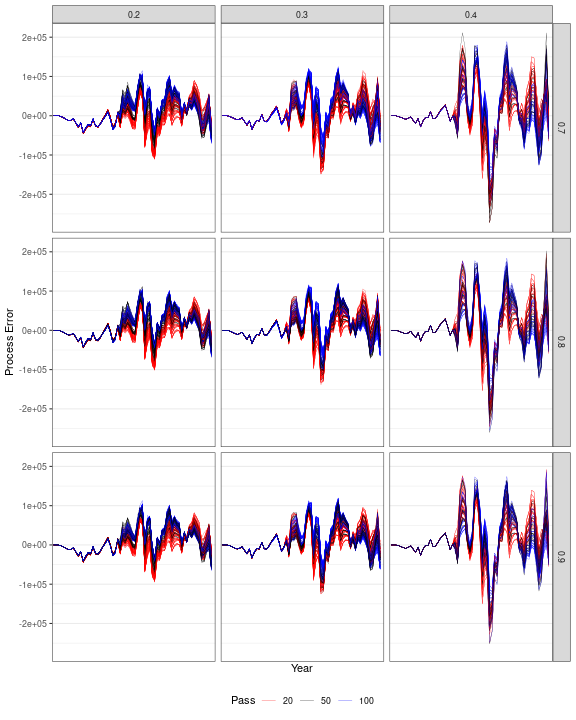
\includegraphics[width=0.75\textwidth]{figures/pf-1.png} 
\caption{Surplus Production by steepness and mature natural mortality}
\label{fig:sp}       
\end{figure}
\fi

